\chapter{Low Frequency Radio Astronomy and the Earth's Ionosphere}\label{Ch:Iono}

\section{Overview}
Beyond the effects of RFI, the Earth's atmosphere has additional impacts on low frequency radio signals from the universe. These impacts come from interactions between the incoming radio signals and the free electrons in the ionosphere. Impacts include refraction and absorption of radio frequency photons. 

These impacts are dependent on the time and geographic location variant structure of the ionosphere. However, in general ionospheric impacts have the potential to mask the \cm signal, as they introduce additional frequency dependent structure into the measured signal. Therefore, it is necessary to quantify and address ionospheric impacts in any \cm measurement. 


\begin{figure}[htb]
\centering
\begin{minipage}[b]{0.48\textwidth}
\centering
\begin{tabular}{|c|c|}
\hline
Layer & Altitude Range (km) \\
\hline
D & 60-100 \\
\hline
E & 100-150 \\
\hline
F1 & 150-250 \\
\hline
F2 & 250-1000+ \\
\hline
\end{tabular}
\caption{Average distribution of the Earth's ionosphere layers.}
\label{Tab:iono_layer}
\vspace{2cm}
\end{minipage}%
\begin{minipage}[b]{0.02\textwidth}
\hspace{1cm}
\end{minipage}%
\begin{minipage}[b]{0.48\textwidth}
\centering
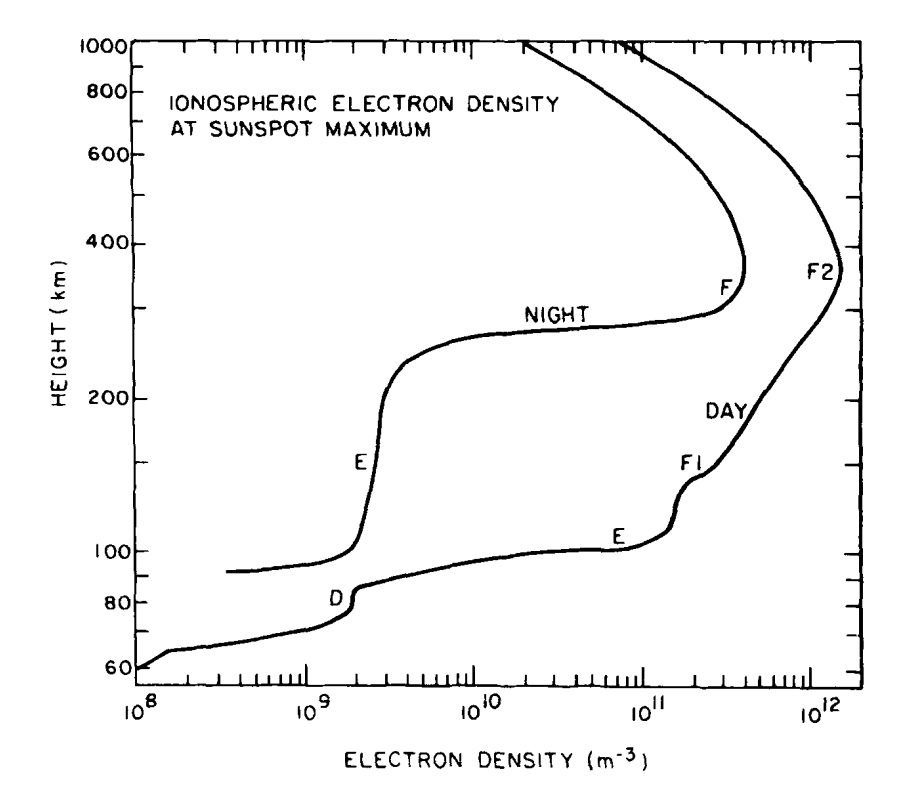
\includegraphics[width=0.95\linewidth]{Ionosphere/figures/atmosphere_layers.jpg}
\caption{Idealized free electron density distribution in Earth's atmosphere showing the ionosphere's layers during day and night. }
\label{Fig:iono_layer}
\end{minipage}
\end{figure}

\section{Earth's Ionosphere}
To understand ionospheric impacts on the \cm signal we need to understand the ionosphere. Earth's ionosphere is located $60 - 1000+$ $km$ above the surface of the Earth and is made up of free electrons and ionized atoms. Neutral atoms in Earth's atmosphere are photoionized by solar radiation, which leads to an altitude dependent distribution of free electrons and ions in the atmosphere.

\subsection{Ionospheric Layers}
This distribution allows us to divide the ionosphere into altitude-dependent regions. The center of each region is defined by a local maximum in the free electrion density distribution as a function of altitude. The regions of the ionosphere are identified in Figure \ref{Tab:iono_layer}. The absolute maximum free electron density ($n_e$) is reached in the F2 layer and is $n_e \cong 10^5 cm^{-3}$ \cite{ionospheres}. 

The presence and width of the ionospheric layers is time dependent and fluctuates over the course of a day. During the day all the layers are present, but during the night some of the layers merge as shown in Figure \ref{Fig:iono_layer}. Electron density distribution also depends on the level of sunspot activity and the specific position (particularly the latitude) on the Earth \cite{thompson_2001}. 

\subsection{Ionosphere Properties}

\subsubsection{Plasma Frequency}
Free electrons in the ionosphere can be treated like a plasma and will modify the propogation of light. We can quantify it by defining a plasma frequency ($\nu_p$), which has a value equal to:

\begin{equation}
\nu_p = \frac{e}{2 \pi} \sqrt{\frac{n_e}{\varepsilon_0 m}} \cong 9 \sqrt{n_e} Hz
\end{equation}

where $n_e$ is in $m^{-3}$ \cite{thompson_2001}. This plasma frequency changes the index of refraction for the ionosphere compared to free space $n = \sqrt{1-\nu_p^2/\nu^2}$, where $\nu$ is the frequency of the light that is passing through the atmosphere \cite{thompson_2001}. 

\subsubsection{Cyclotron Frequency}
In addition to the plasma frequency due to free electrons, a static magnetic field in the ionsphere will lead to motion of the free electrons. This motion can be quantified using a gyrofrequency defined as ($\nu_B = eB/2 \pi m$), and has a typical magnitude of $\nu_B \cong 1.4 MHz$ \cite{thompson_2001}. 

In adding in the cyclotron frequency to the index of refraction, the direction of the magnetic field with respect to the incoming signal matters. This means that the impact of a static magnetic field will be polarized. This is the source of Faraday roation in Earth's atmosphere \cite{thompson_2001}. However, since the impact is proportional to $\nu_B/\nu$ and $\nu \gg \nu_B$ for our frequency band; we will neglect the impact from the Earth's magnetic field in the rest of the discussion. 


\begin{figure}[htb]
\begin{center}
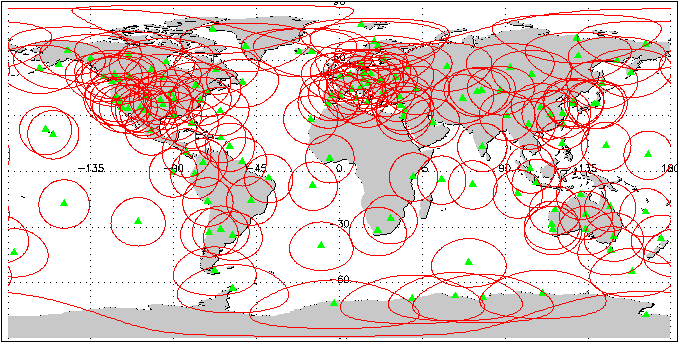
\includegraphics[width=0.95\linewidth]{Ionosphere/figures/gps_sitemap.png}
\caption{Global Map of GPS Network stations used for the quasi-real time maps of $TEC$ available online at (iono.jpl.nasa.gov)}
\label{Fig:gps_stat}
\end{center}
\end{figure}

\begin{figure}[htb]
\centering
\begin{minipage}[b]{0.48\textwidth}
\centering
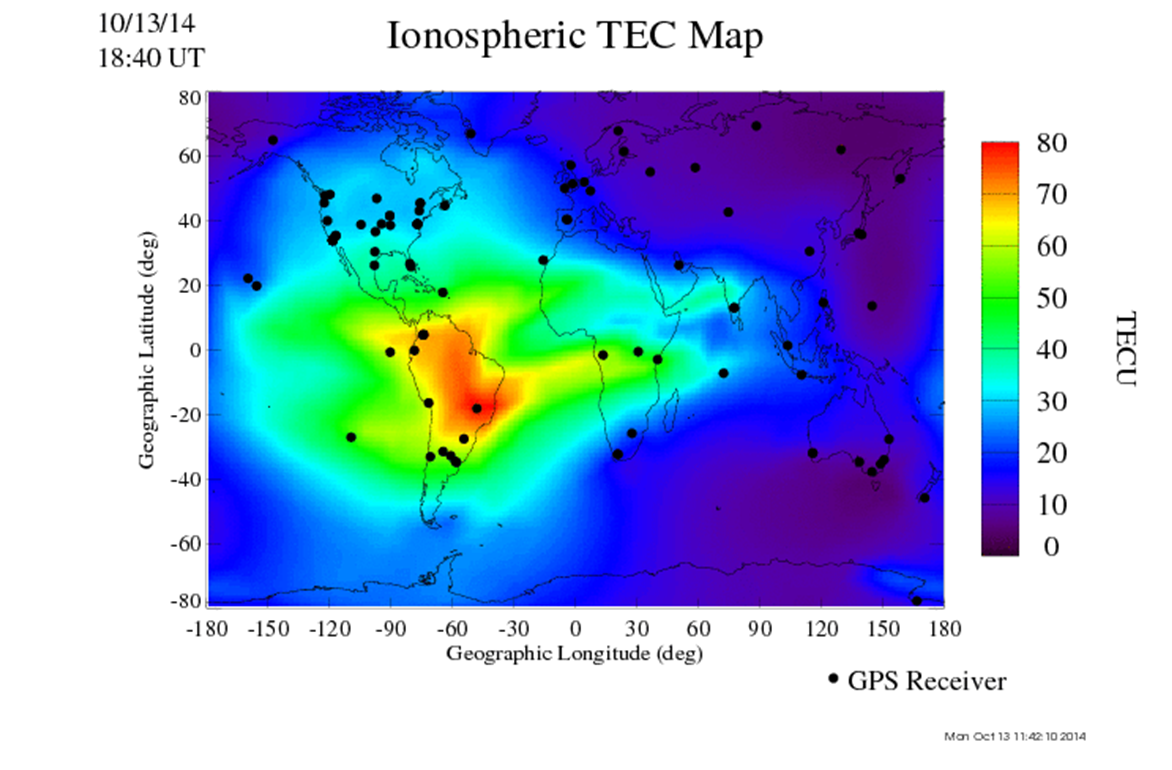
\includegraphics[width=0.95\linewidth]{Ionosphere/figures/TEC_map_20141013_18-40UT.png}
\caption{$TEC$ map for October 13th, 2014 at 18:40 UTC. (iono.jpl.nasa.gov)  }
\label{Fig:fall_tec_global}
\end{minipage}%
\begin{minipage}[b]{0.02\textwidth}
\hspace{1cm}
\end{minipage}%
\begin{minipage}[b]{0.48\textwidth}
\centering
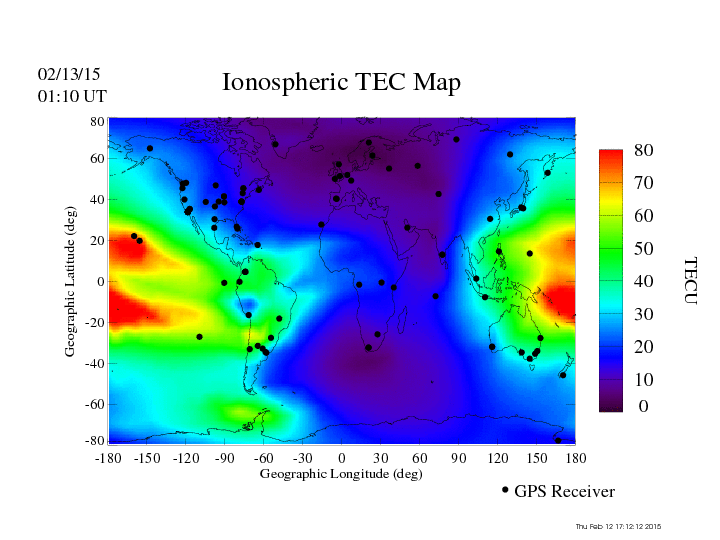
\includegraphics[width=0.95\linewidth]{Ionosphere/figures/TEC_map_20150213_01-10UT.png}
\caption{$TEC$ map for February 13th, 2015 at 01:10 UTC. (iono.jpl.nasa.gov)  }
\label{Fig:winter_tec_global}
\end{minipage}
\end{figure}

\section{Total Electron Content}
Measurement of the number of free electrons at a given altitude ($n_e$) can be quite difficult. Instead, scientists typically measure the total electron content ($TEC$). $TEC$ is the integrated number of free electrons for a skewer through the atmosphere. It is defined as:

\begin{equation}
TEC = \int_0^\infty n_e (h) dh 
\end{equation}

where $h$ is the altitude \cite{thompson_2001}. $TEC$ is typically quoted in $TECU$, where $1 TECU$ corresponds to an average $n_e = 10^{16}$ electrons per $m^2$ \cite{vedantham_2014}. Total electron content is continually monitored on Earth using measurements from GPS stations around the world. This data is collected by a number of agencies that convert the data into maps. 

\subsection{Measuring $TEC$}
Real time maps of $TEC$ over the entire world are made by NASA JPL using the GPS stations shown in Figure \ref{Fig:gps_stat} and are available online\footnote{\url{http://iono.jpl.nasa.gov/latest_rti_global.html}}. The plots are based on a five minute average, and the image is updated online every five minutes. A couple of examples of these maps are Figures \ref{Fig:fall_tec_global} and \ref{Fig:winter_tec_global}, which show the measured $TEC$ distribution for two different times of day (and times of year). The bright region with high $TEC$ corresponds to the part of the globe currently receiving sunlight. Also, areas close to the equator are much brighter than areas near the poles in both the day and night regions.

\begin{figure}[htb]
\centering
\begin{minipage}[b]{0.48\textwidth}
\centering
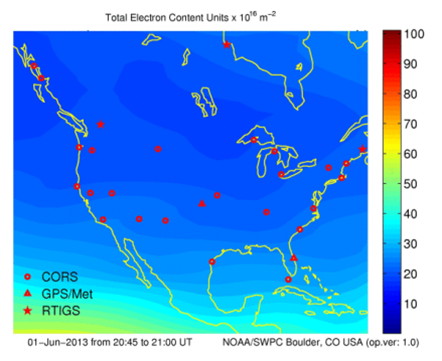
\includegraphics[width=0.95\linewidth]{Ionosphere/figures/NA_TEC_day.png}
\caption{North American TEC map for June 1st, 2013 at 21:00 UTC. (www.swpc.noaa.gov)   }
\label{Fig:day_TEC_NA}
\end{minipage}%
\begin{minipage}[b]{0.02\textwidth}
\hspace{1cm}
\end{minipage}%
\begin{minipage}[b]{0.48\textwidth}
\centering
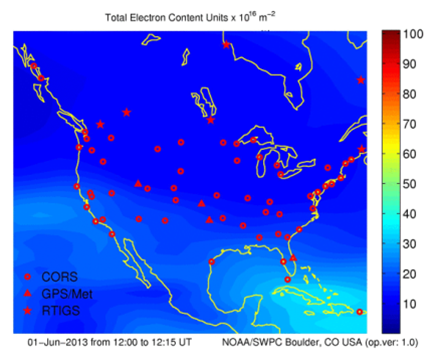
\includegraphics[width=0.95\linewidth]{Ionosphere/figures/NA_TEC_night.png}
\caption{North American TEC map for June 1st, 2013 at 12:15 UTC. (www.swpc.noaa.gov) }
\label{Fig:night_TEC_NA}
\end{minipage}
\end{figure}

In addition, the Space Weather Prediction Center of the National Oceanic and Atmospheric Administration (NOAA) has a model for $TEC$ in North America based on a subset of the GPS stations\footnote{\url{http://www.swpc.noaa.gov/products/us-total-electron-content}}. Beyond images, the data is also available online for the most recent few days of data. Using archive data, we can see plots of North American TEC for the Isla Guadalupe deployment in June 2013, as shown in Figures \ref{Fig:day_TEC_NA} and \ref{Fig:night_TEC_NA}. 


\begin{figure}[htb]
\begin{center}
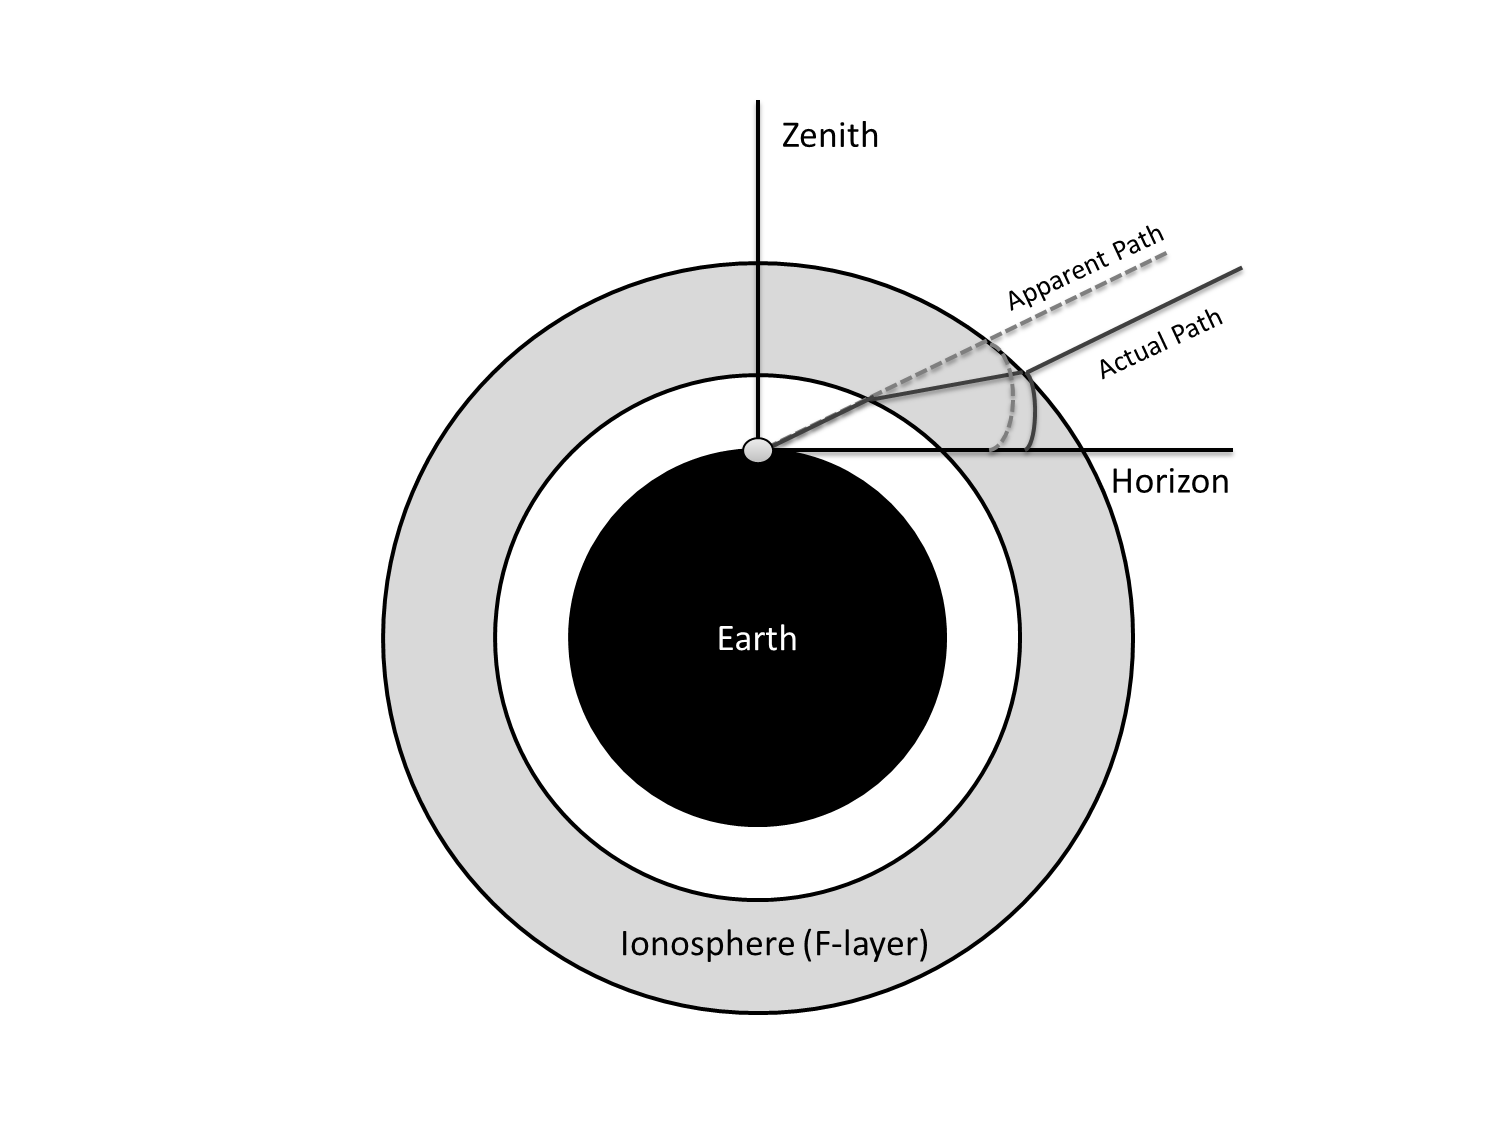
\includegraphics[width=0.95\linewidth]{Ionosphere/figures/refraction.png}
\caption{Ray tracing for incident light with a single ionospheric layer. Sizes are not to scale. }
\label{Fig:iono_refrac}
\end{center}
\end{figure}

\section{Ionospheric Impacts}

\subsection{Refraction}
From basic optics, Snell's law tells us that light passing through an interface between materials having different indices of refraction will be bent. The magnitude of this bending depends only on the difference between the indices of the two materials and the incidence angle of the light ($n_0 sin \theta_0 = n_1 sin \theta_1$). If light passes through a flat plane of material with index $n_1$, having air ($n=1$) on either side, the angle of the light doesn't change. However, the ionosphere is a set of spherical layers rather than a flat plane \cite{thompson_2001}. 

Therefore, when light enters the ionosphere at some angle $\theta_0 \neq 0$, the light reaches the ground with an apparent incident angle that differs from its actual incident angle. This is shown in Figure \ref{Fig:iono_refrac}, where I've used a single ionospheric layer for simplicity. We can define the difference of angle $\delta \theta = \theta_{apparent}-\theta{actual}$ \cite{thompson_2001}.


\begin{figure}[htb]
\begin{center}
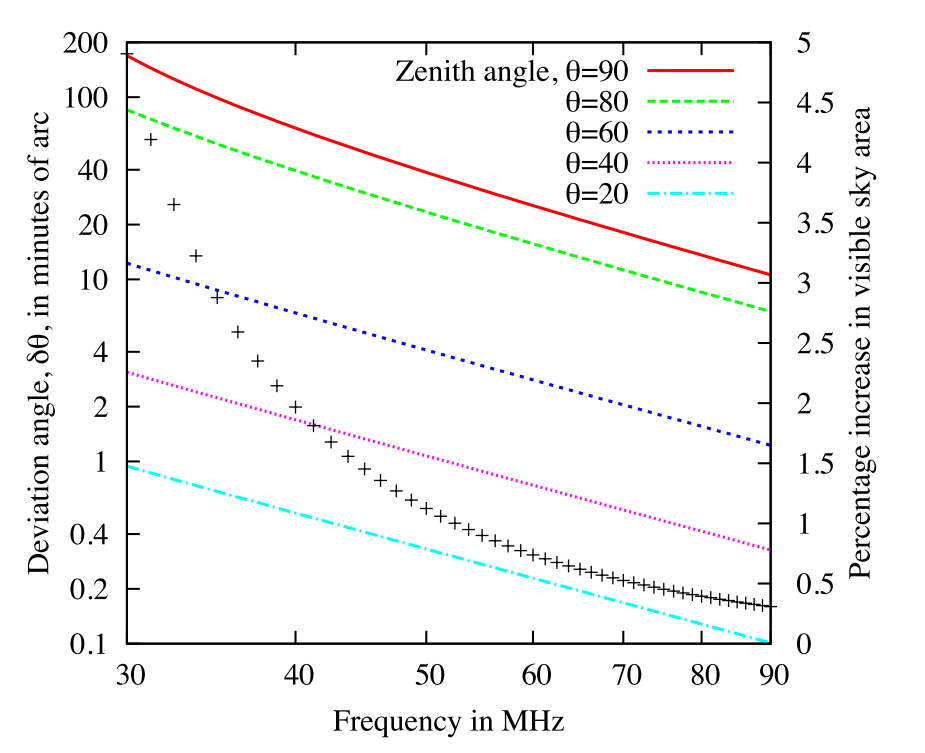
\includegraphics[width=0.95\linewidth]{Ionosphere/figures/refraction_impact.jpg}
\caption{Refraction angle ($\delta \theta$) for $TEC= 10 TECU$ as a function of zenith angle and frequency from Vedantham et al \cite{vedantham_2014}.}
\label{Fig:refrac_est}
\end{center}
\end{figure} 

To compute $\delta \theta$ requires a model for the ionosphere. The simplest approximation is a single ionospheric layer with constant $n_e$. Using this approximation, $\delta \theta \propto \nu^{-2} cos(\theta)(sin^2 \theta + 2 h_F/R_e)^{-1.5}$, where $h_F$ is the mean height of the ionosphere and $R_e$ is the Earth's radius. Vedantham et al \cite{vedantham_2014} used this approximation, assuming that the total electron content was $10 TECU$ and $h_F = 300 km$, to calculate the deviation angle $\delta \theta$ and percentage increase in visible sky area (beyond the normal horizon). This is shown in Figure \ref{Fig:refrac_est}. 


\subsection{Absorption}


